\begin{figure}[h]
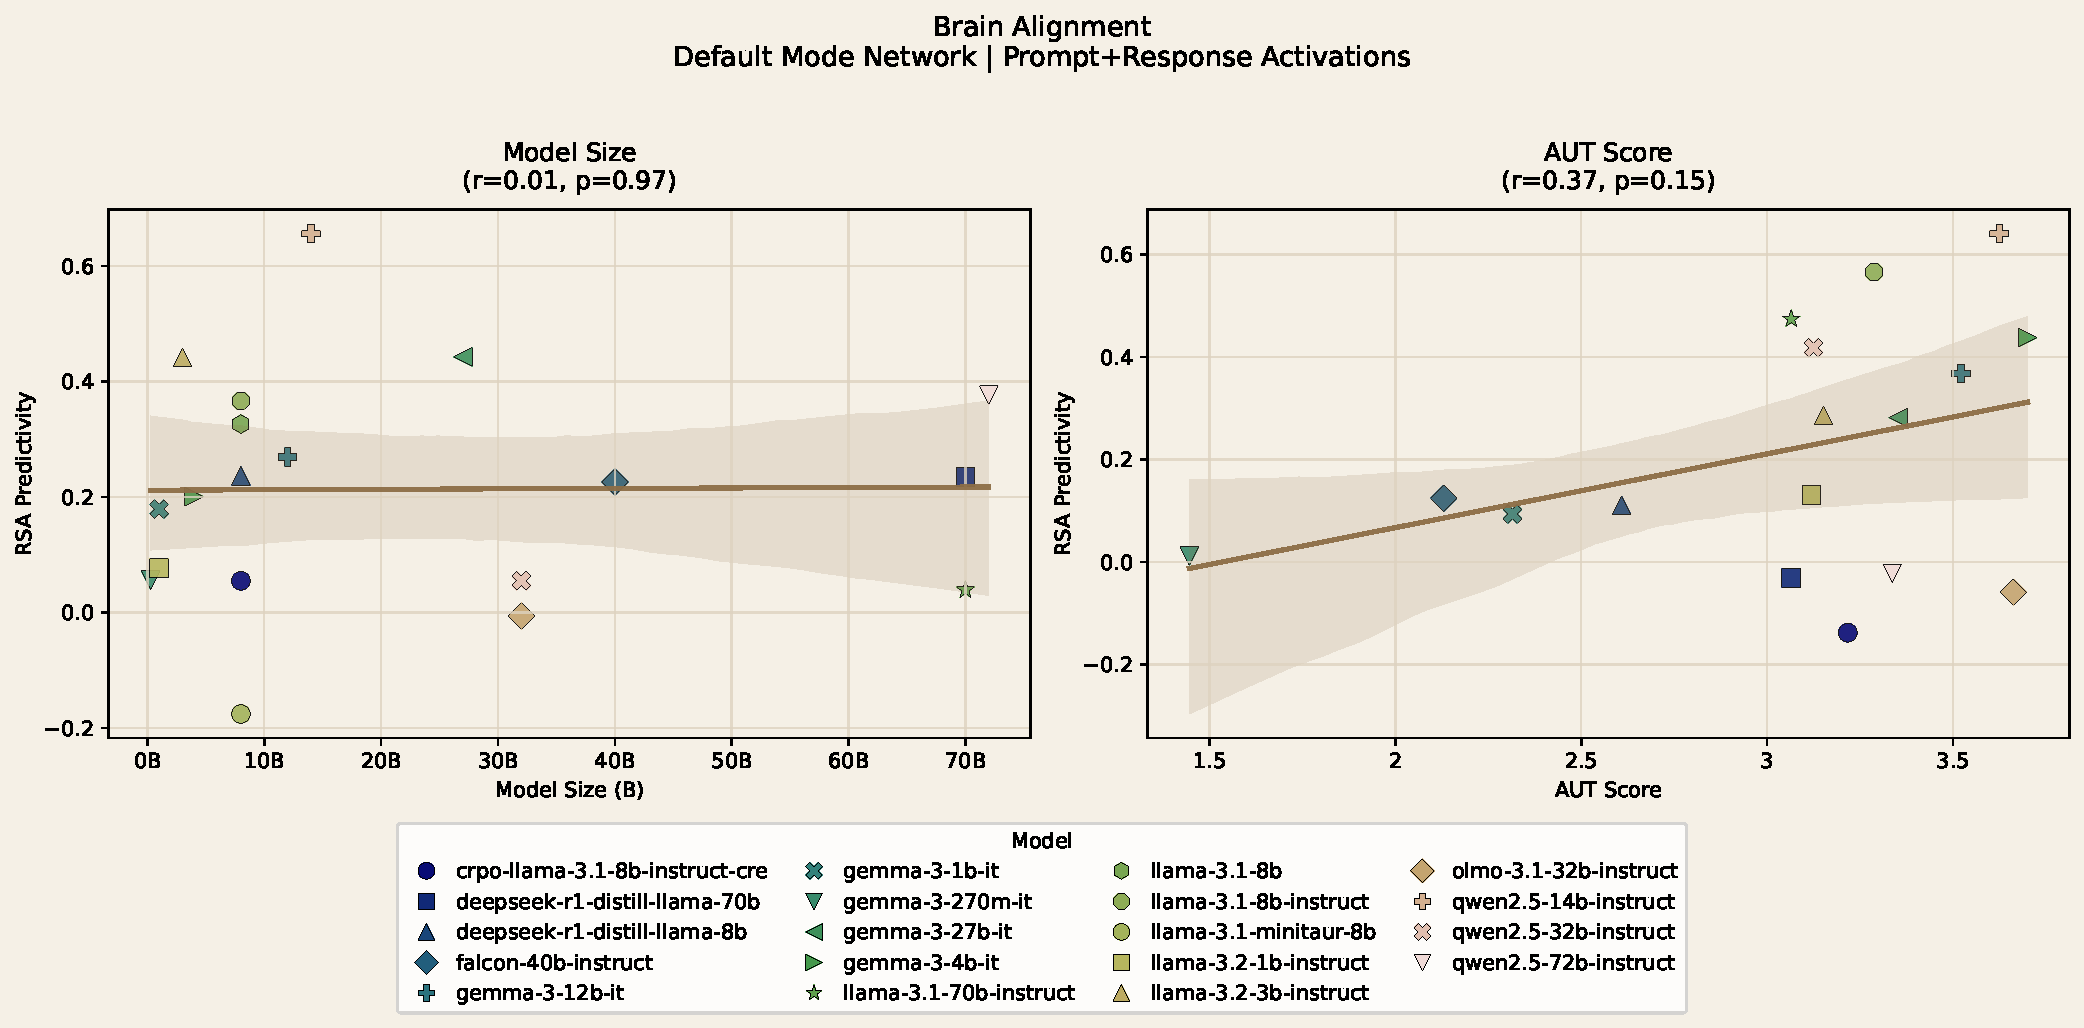
\includegraphics[width=\linewidth]{figures/main_results_yeo_dmn_model_resp_nc0_t_1_t_mean.pdf}
\centering
\caption{\textbf{Default Mode Network (DMN) AUT brain alignment results by model size and task performance using model activations on stimuli (prompt) and model response.} $r$ and $p$ correspond to the Pearson correlation coefficient and p-value.}
\label{fig:alignment-aut-yeo-dmn-response}
\end{figure}

\begin{figure}[h]
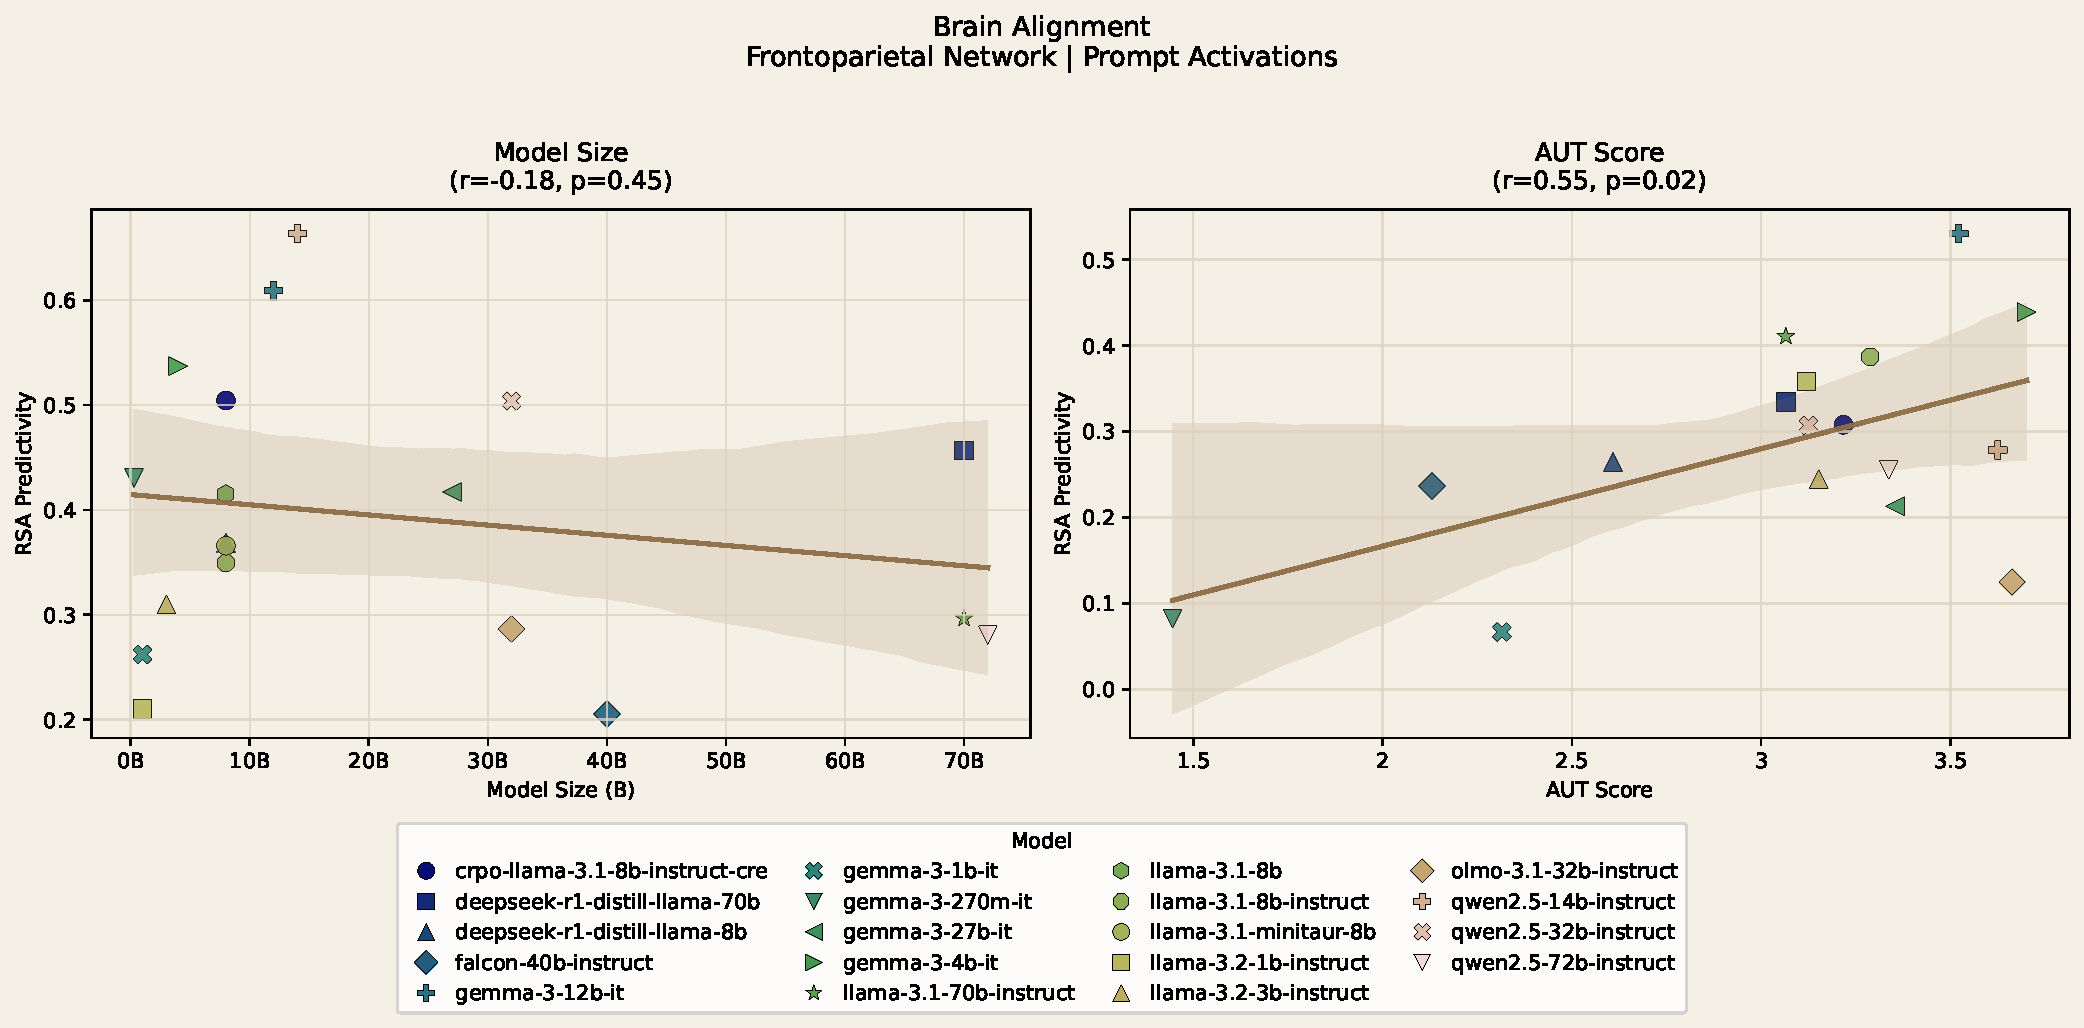
\includegraphics[width=\linewidth]{figures/main_results_yeo_fp_prompt_nc0_t_1_t_mean.pdf}
\centering
\caption{\textbf{Frontoparietal Network (FPN) AUT brain alignment results by model size and task performance using model activations on stimuli (prompt) only.} $r$ and $p$ correspond to the Pearson correlation coefficient and p-value.}
\label{fig:alignment-aut-yeo-fp-prompt}
\end{figure}

\begin{figure}[h]
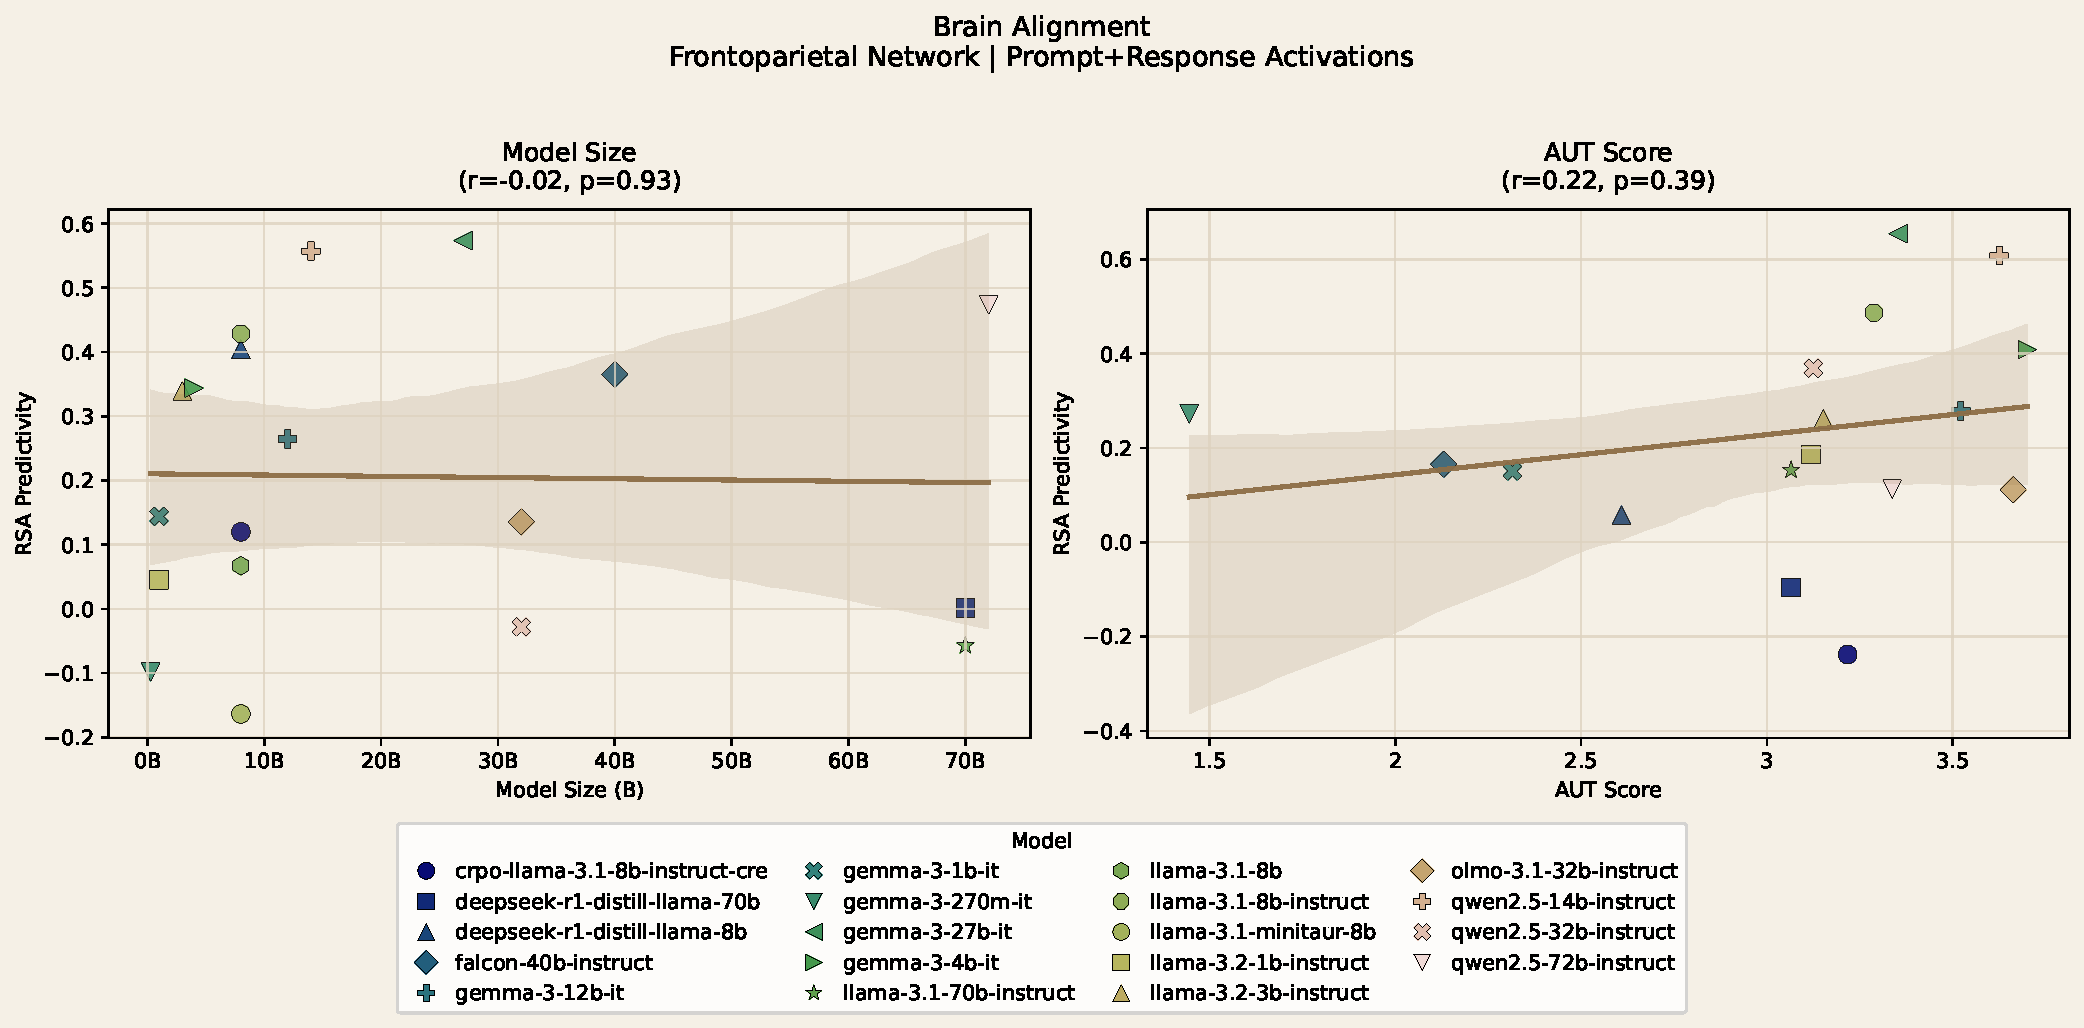
\includegraphics[width=\linewidth]{figures/main_results_yeo_fp_model_resp_nc0_t_1_t_mean.pdf}
\centering
\caption{\textbf{Frontoparietal Network (DMN) AUT brain alignment results by model size and task performance using model activations on stimuli (prompt) and model response.} $r$ and $p$ correspond to the Pearson correlation coefficient and p-value.}
\label{fig:alignment-aut-yeo-fp-response}
\end{figure}

\begin{figure}[h]
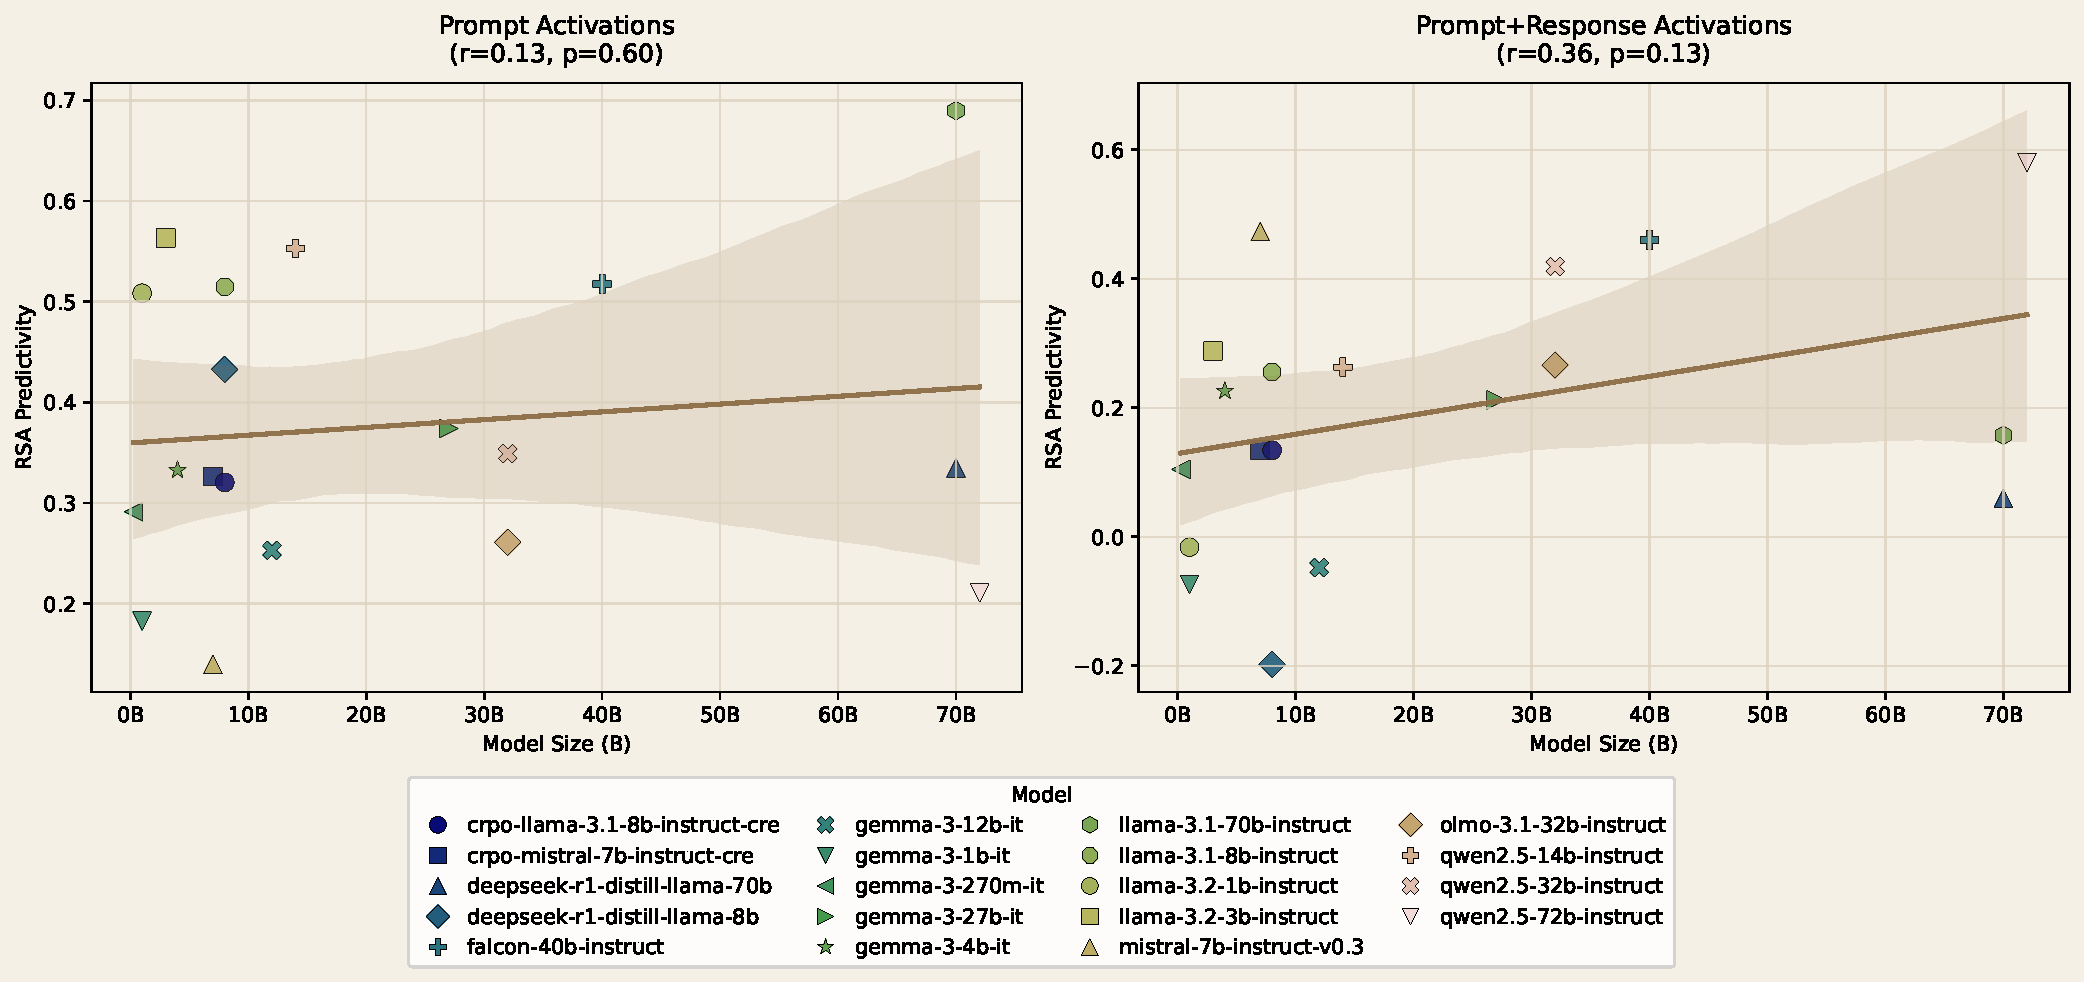
\includegraphics[width=\linewidth]{figures/model_size_res_yeo_dmn_oct_nc0_t_1.pdf}
\centering
\caption{\textbf{Default Mode Network (DMN) OCT brain alignment results by model size on both stimuli (prompt) only and stimuli+model response activations.} $r$ and $p$ correspond to the Pearson correlation coefficient and p-value.}
\label{fig:alignment-oct-model-size-yeo-dmn}
\end{figure}

\begin{figure}[h]
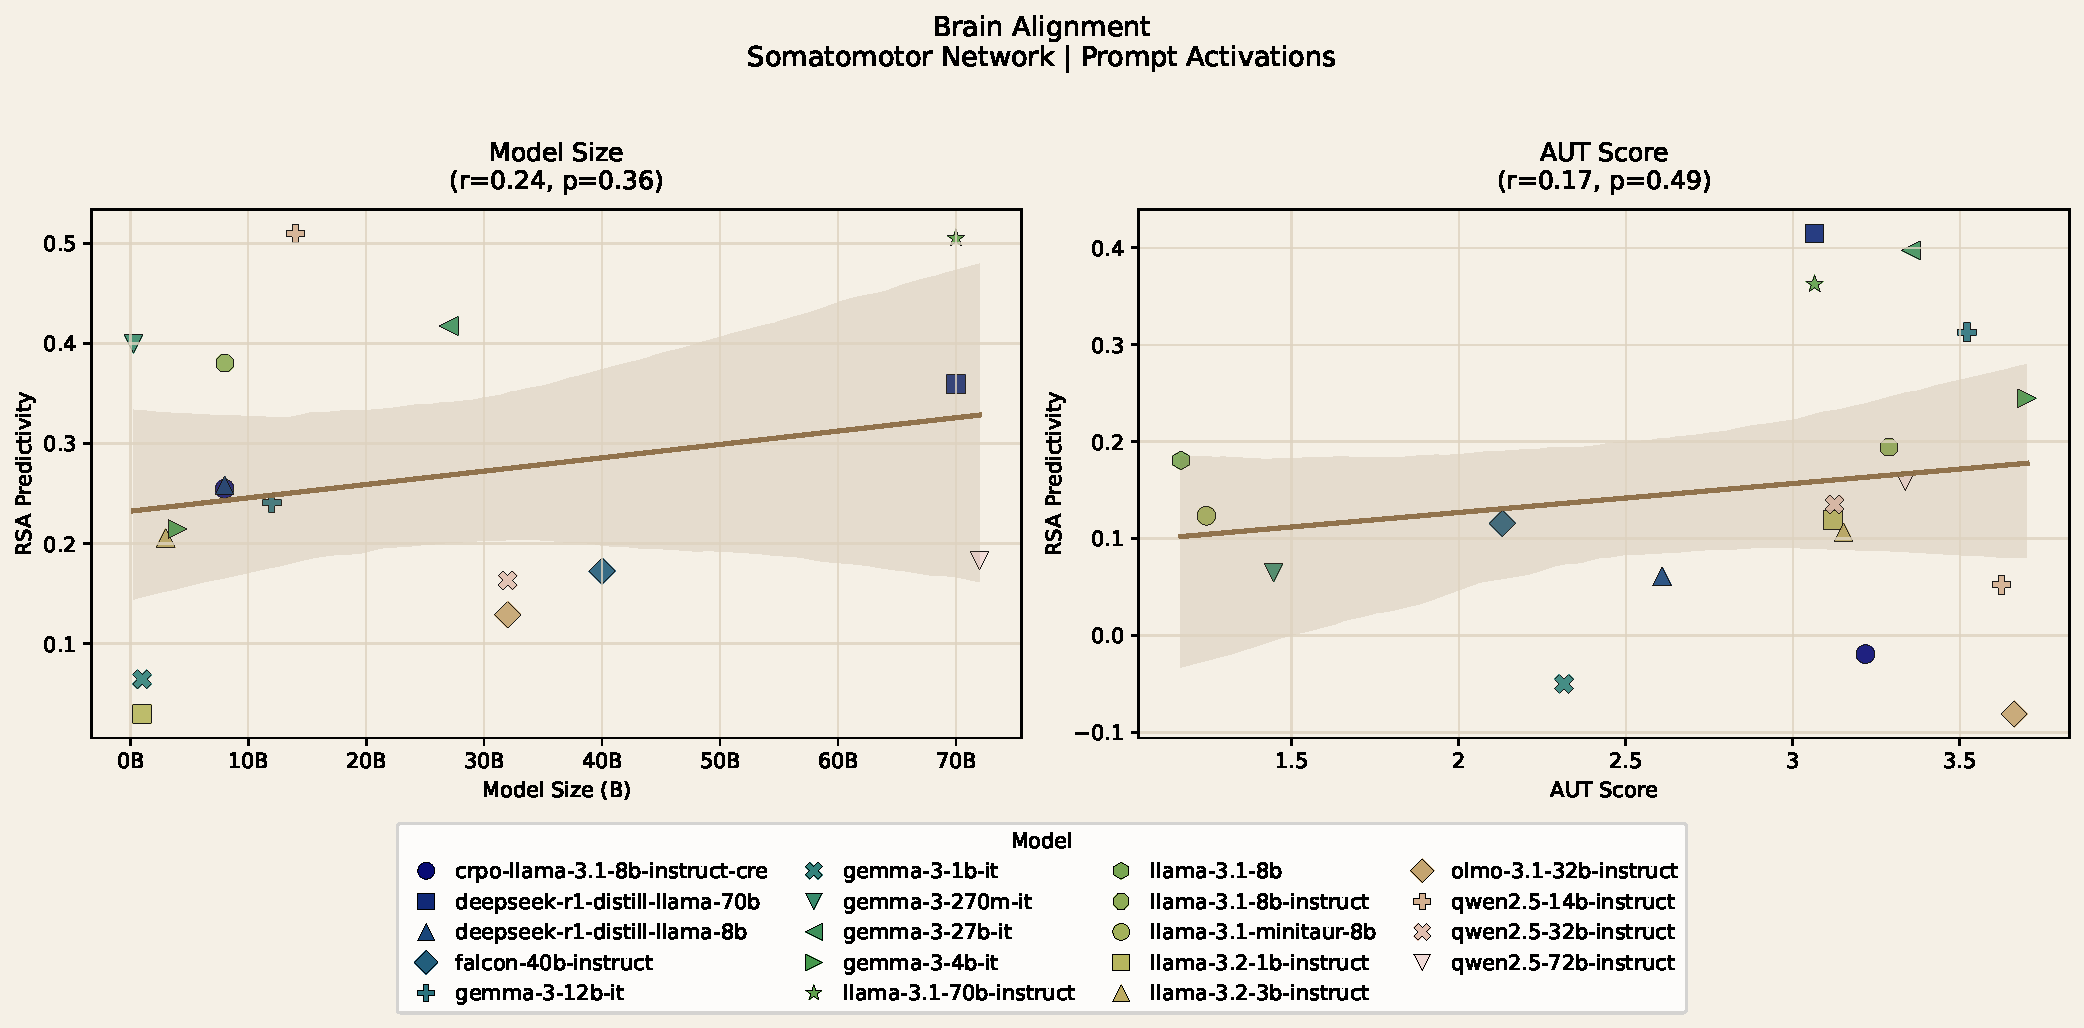
\includegraphics[width=\linewidth]{figures/main_results_yeo_som_prompt_nc0_t_1_t_mean.pdf}
\centering
\caption{\textbf{Somatomotor Network (SOM) AUT brain alignment results by model size and task performance using model activations on stimuli (prompt) only.} $r$ and $p$ correspond to the Pearson correlation coefficient and p-value.}
\label{fig:alignment-aut-yeo-som-prompt}
\end{figure}

\begin{figure}[h]
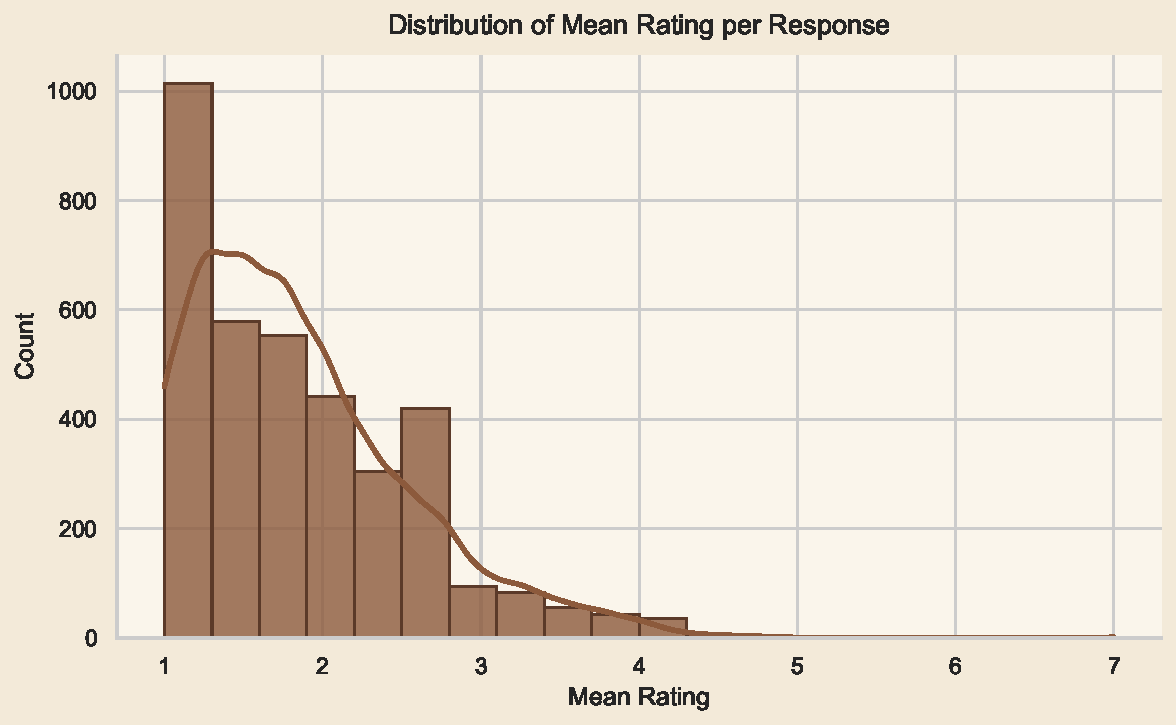
\includegraphics[width=\linewidth]{figures/mean_rating_distribution.pdf}
\centering
\caption{Distribution of mean AUT ratings per human response.}
\label{fig:dist-mean-rating}
\end{figure}

\begin{prompt}[title={Modified AUT Instructions for scoring}, label=prompt:aut_instructions_scoring]
\begin{Verbatim}[breaklines, breaksymbol={}]
Think of creative uses for objects. Report only the most original idea in a few words.
\end{Verbatim}
\end{prompt}

\begin{prompt}[title={Modified OCT Instructions for scoring}, label=prompt:oct_instructions_scoring]
\begin{Verbatim}[breaklines, breaksymbol={}]
Think of the physical properties of objects. Report only the most prominent characteristic in a few words.
\end{Verbatim}
\end{prompt}